\section{Final Long Short-Term Memory Recurrent Neural
Network}\label{sec:rnnfinalrnn}

The final RNN is shown in \lstref{lst:finalrnn}.

\lstinputlisting[language={matlab}, label={lst:finalrnn},
style={Matlab-editor}, basicstyle={\footnotesize\ttfamily}, caption={The final
RNN architecture and training options.}]{rnndef.m}

This network has been trained for \(350\) epochs. Training ended after
\(33337\) iterations (\(238\) epochs plus some iterations), due to validation
loss not improving anymore. The network achieved excellent results with \(R >
0.99\) for all sets. Complete results are shown in \lstref{lst:rnnresults}.
\figref{fig:rnnregression} shows the regression plots for the RNN.
\figref{fig:rnnpredictions} shows an example of how the RNN predicts values for
the ECG.

\lstinputlisting[language={}, label={lst:rnnresults},
caption={Results of the final Long Short-Term Memory Recurrent Neural
Network.}]{rnnresults.txt}

\begin{figure}[htbp]
	\centering
	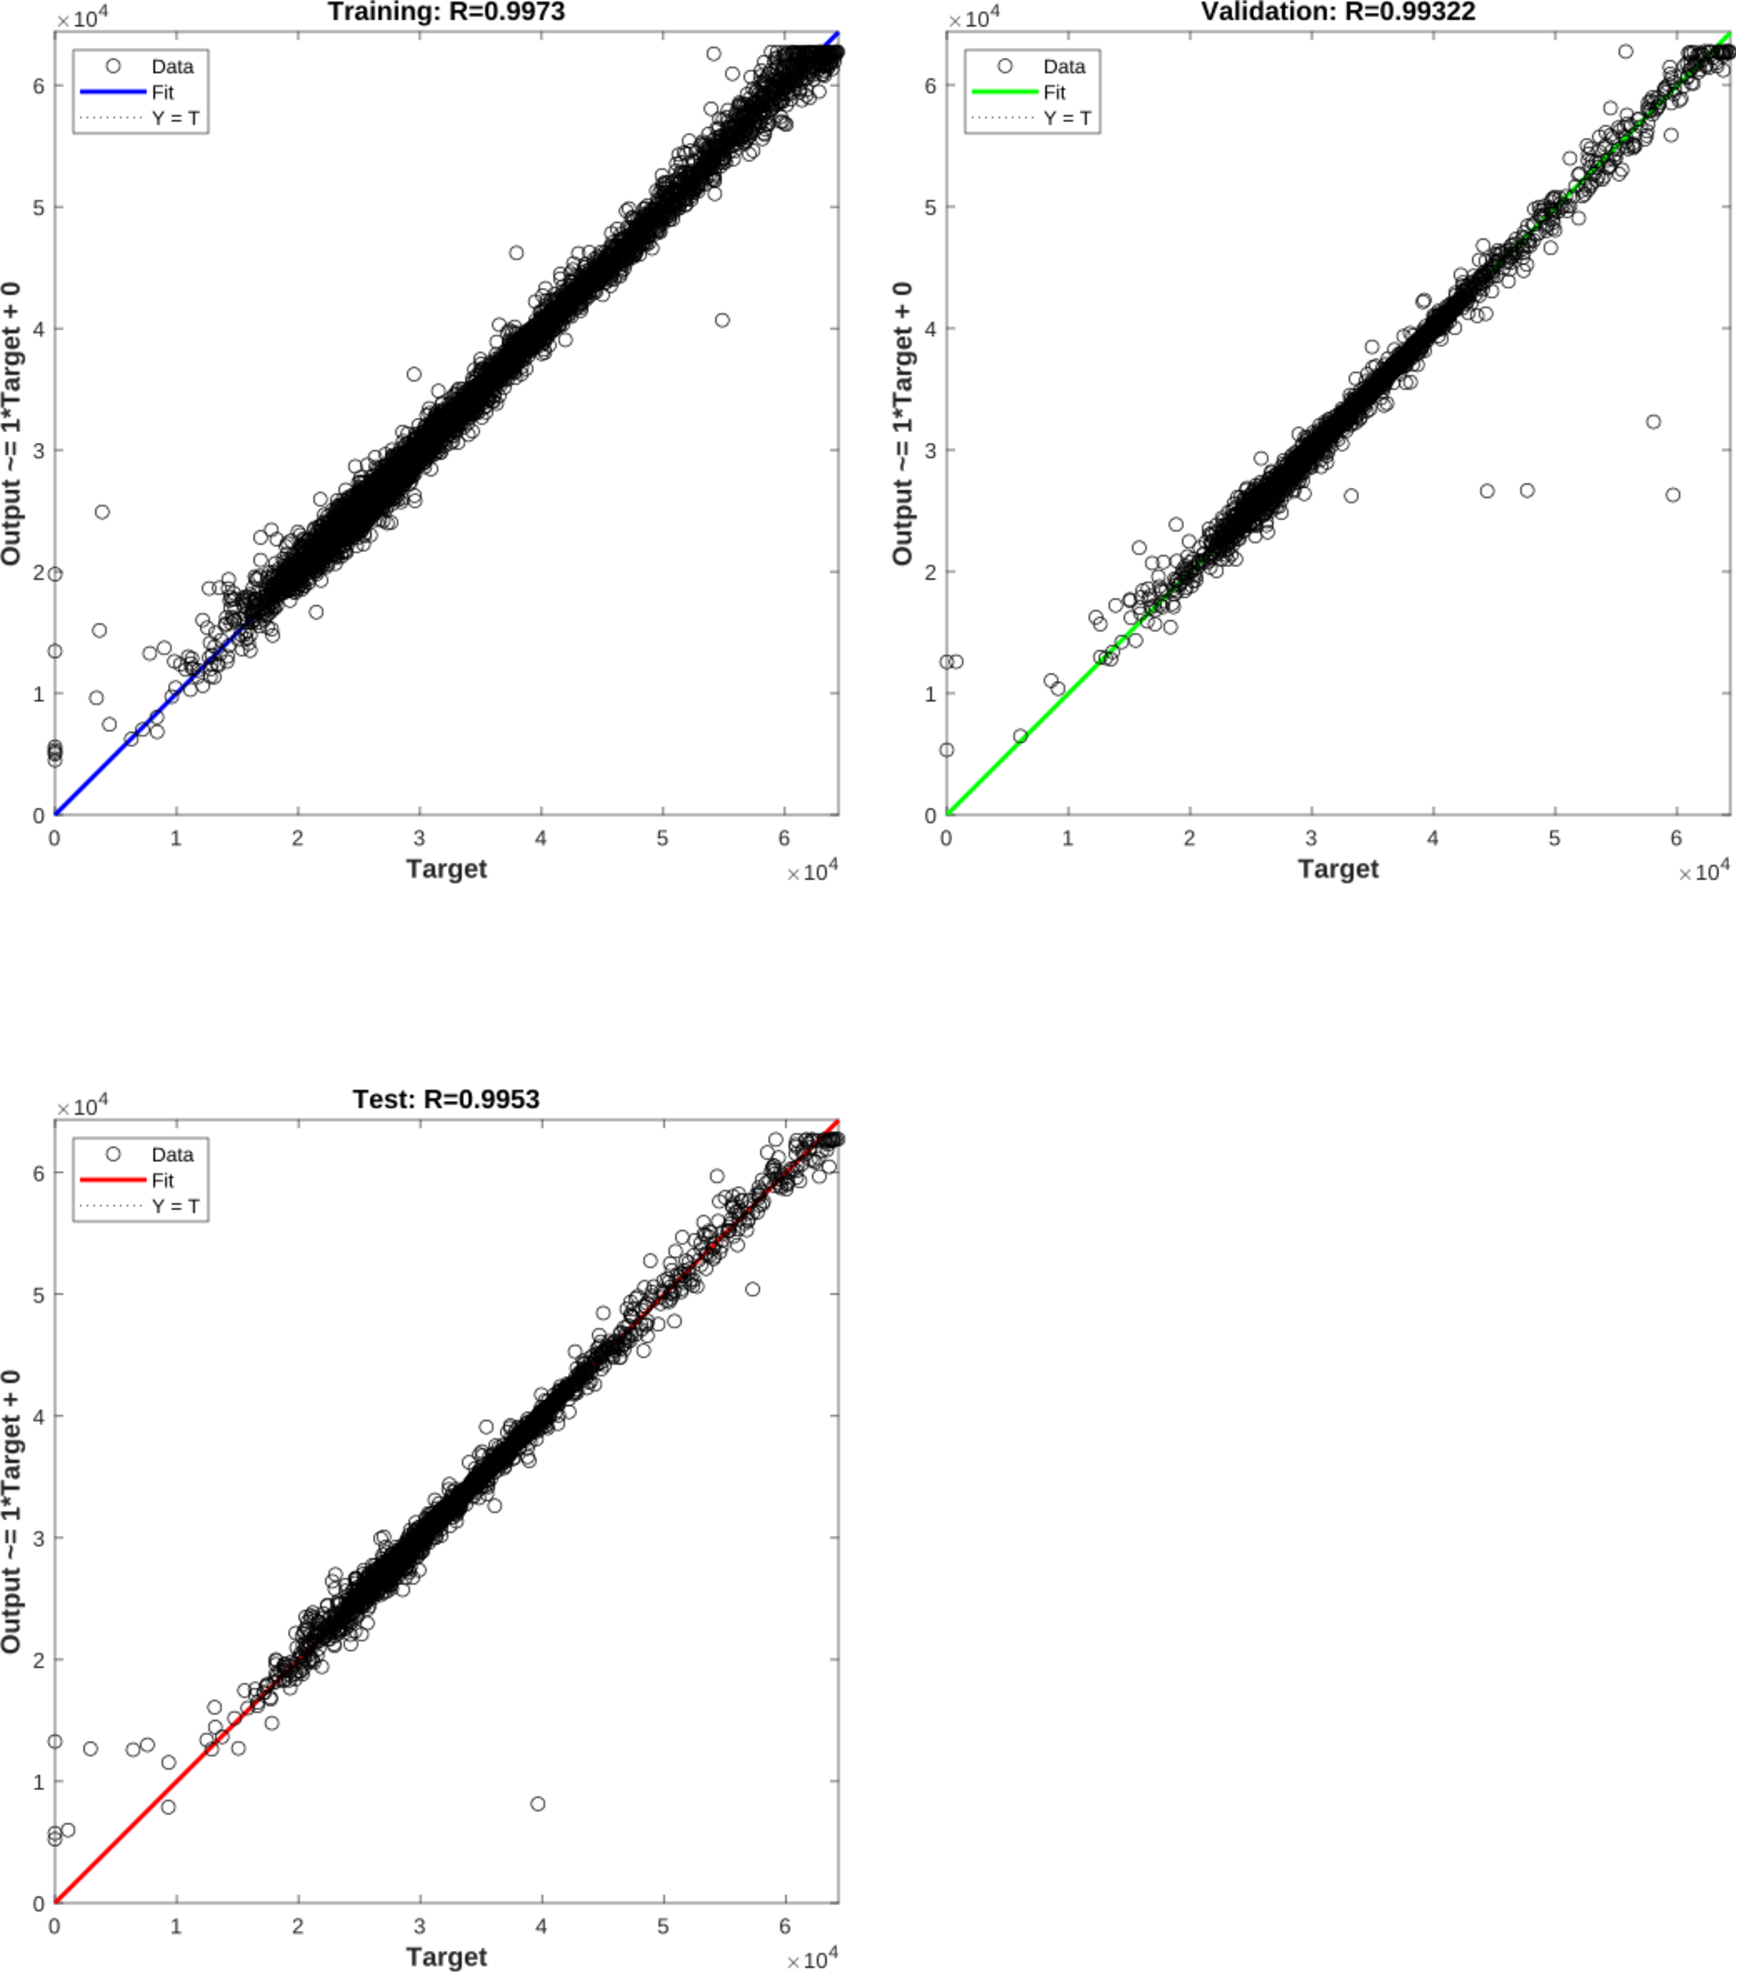
\includegraphics[width=\textwidth]{rnnregression}
	\caption{Regression plots for all three sets for the LSTM RNN
	that predicts values for the ECG.}\label{fig:rnnregression}
\end{figure}

\begin{figure}[htbp]
	\centering
	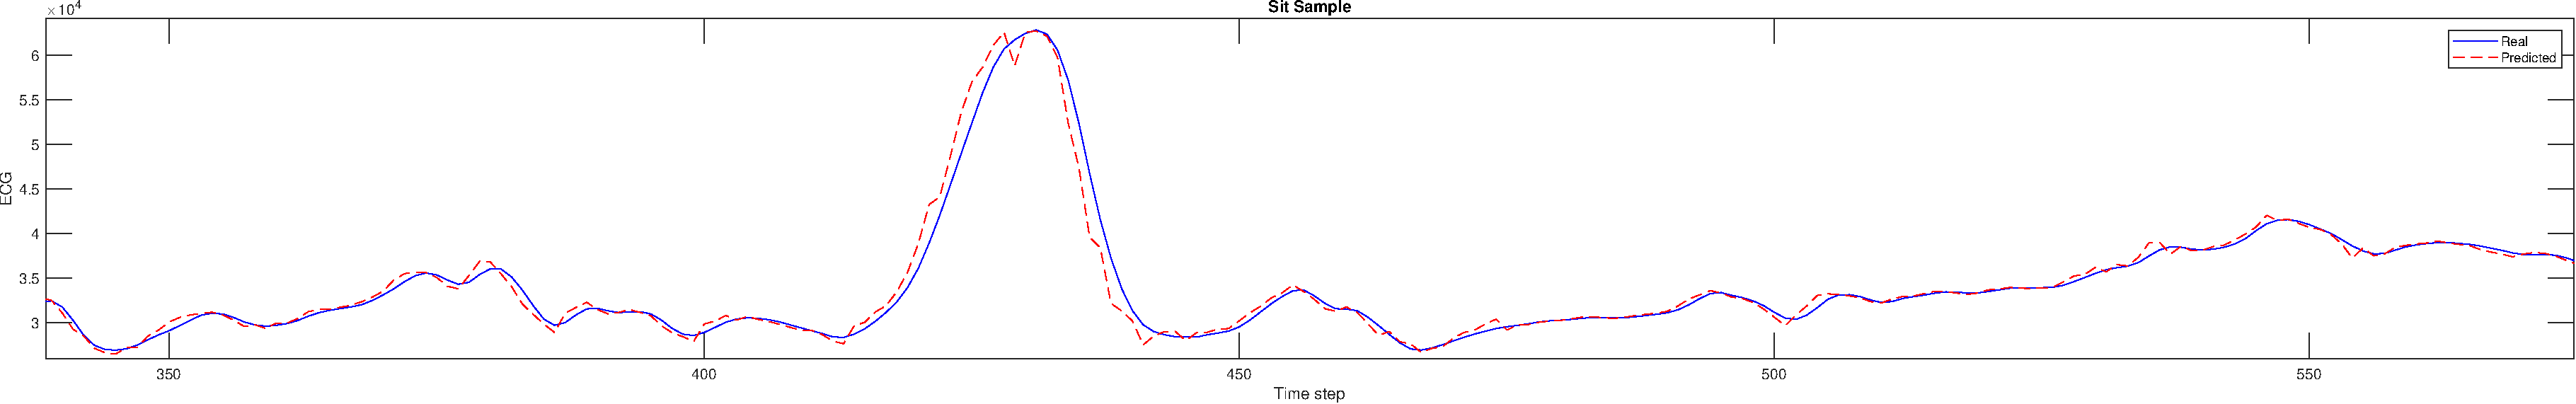
\includegraphics[width=\textwidth]{rnnpredictions}
	\caption{The 2 lines nearly overlap each other, proving that the RNN
	performs very well (zoom: this is vector
	graphics).}\label{fig:rnnpredictions}
\end{figure}
